% Jason R. Blevins - Curriculum Vitae
%
% Copyright (C) 2004-2014 Jason R. Blevins <jrblevin@sdf.org>
% http://jblevins.org/
%
% You may use use this document as a template to create your own CV
% and you may redistribute the source code freely.  No attribution is
% required in any resulting documents.  I do ask that you please leave
% this notice and the above URL in the source code if you choose to
% redistribute this file.

\documentclass[11pt,letterpaper]{article}

\usepackage{hyperref}
\hypersetup{colorlinks,linkcolor={blue},citecolor={blue}}
\usepackage{geometry}
\usepackage{fontawesome}
% Underline vertical space
\usepackage{soul}
        \setul{0ex}{}

% Fonts
\usepackage[T1]{fontenc}
\usepackage{times}
%\usepackage[urw-garamond]{mathdesign}
\usepackage{graphicx}
\usepackage{natbib}
\usepackage{bibentry}
\bibliographystyle{plainnat}

% Set your name here
\def\name{CV - Leimin Tian}

% The following metadata will show up in the PDF properties
\hypersetup{
  colorlinks = true,
  urlcolor = blue,
  pdfauthor = {Leimin Tian},
  pdfkeywords = {Leimin Tian, CV},
  pdftitle = {CV - Leimin Tian - 2024},
  pdfsubject = {CV - Leimin Tian - 2024},
  pdfpagemode = UseNone
}

\geometry{
  body={6.5in, 9.0in},
  left=1.0in,
  top=1.0in
}

% Customize page headers
\pagestyle{myheadings}
\markright{\name}
\thispagestyle{empty}

% Custom section fonts
\usepackage{sectsty}
\sectionfont{\rmfamily\mdseries\Large}
\subsectionfont{\rmfamily\mdseries\itshape\large}

% Other possible font commands include:
% \ttfamily for teletype,
% \sffamily for sans serif,
% \bfseries for bold,
% \scshape for small caps,
% \normalsize, \large, \Large, \LARGE sizes.

% Don't indent paragraphs.
\setlength\parindent{0em}

% Make lists without bullets and compact spacing
%\renewenvironment{itemize}{
%  \begin{list}{}{
%    \setlength{\leftmargin}{1.5em}
%    \setlength{\itemsep}{0.25em}
%    \setlength{\parskip}{0pt}
%    \setlength{\parsep}{0.25em}
%  }
%}{
%  \end{list}
%}

\begin{document}

\nobibliography{MyPaperList}

{\huge Dr Leimin Tian \\}
\smallskip

\begin{minipage}[b]{0.5\textwidth}
  Senior Scientist \& Team Leader\\
  Human-Robot Interaction Team, \href{https://research.csiro.au/robotics/}{Robotics Group}\\
  Data61, CSIRO\\
  \\Adjunct Senior Lecturer\\
  \href{https://www.monash.edu/engineering/robotics}{Robotics}, ECSE, Engineering\\
  % \href{https://www.monash.edu/it/hcc/human-centred-ai-lab}{Human-Centered AI Lab} \\
  % \href{https://www.monash.edu/data-futures-institute}{Data Futures Institute} \\
  Monash University
  % Melbourne, Australia \\
  % Phone: (+61) (0) 432 987 082 \\
  % Email: \href{mailto:Leimin.Tian@data61.csiro.au}{Leimin.Tian@data61.csiro.au} \\
  % ORCID: \href{https://orcid.org/0000-0001-8559-5610}{0000-0001-8559-5610}\\
  % Other: \href{https://tianleimin.github.io/}{Personal Page}, \href{https://scholar.google.com/citations?hl=en&user=d-PQpWgAAAAJ&view_op=list_works&sortby=pubdate}{Google Scholar}, \href{https://twitter.com/LeiminTian}{Twitter}
\end{minipage}
\hfill
\begin{minipage}[b]{0.45\textwidth}
  Melbourne, Australia \\
  Phone: (+61) (0) 432 987 082 \\
  Emails:\\
  \hspace*{1em}\href{mailto:Leimin.Tian@data61.csiro.au}{Leimin.Tian@data61.csiro.au} \\
  \hspace*{1em}\href{mailto:Leimin.Tian@monash.edu}{Leimin.Tian@monash.edu} \\
  ORCID: \href{https://orcid.org/0000-0001-8559-5610}{0000-0001-8559-5610}\\
  Other: \href{https://tianleimin.github.io/}{Personal Page}, \href{https://scholar.google.com/citations?hl=en&user=d-PQpWgAAAAJ&view_op=list_works&sortby=pubdate}{Google Scholar}, \href{https://twitter.com/LeiminTian}{Twitter}
\end{minipage}
% \begin{minipage}[b]{0.4\textwidth}
%   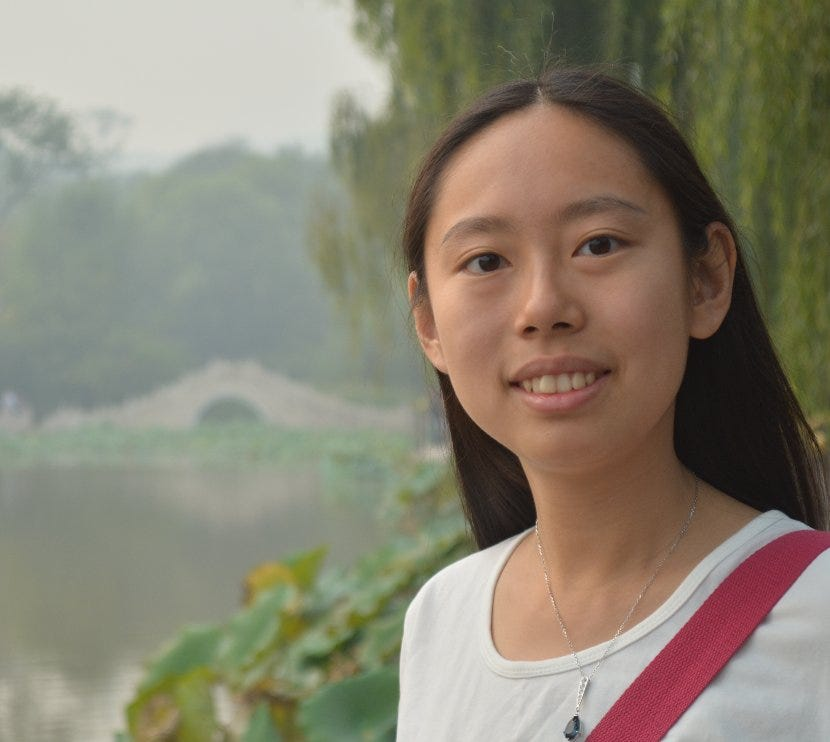
\includegraphics[width=\textwidth]{LeiminTian}
% \end{minipage}

\smallskip

\subsection*{Research Interests}
Human-Robot Interaction and collaboration, Human-Robot Teaming, Affective Computing, Social Robotics, Human-Centred AI, Multimodal Behavioural Analytics, Digital Health, Dialogue Systems

\subsection*{Education}
\begin{itemize}
  \item Ph.D. in Informatics. The University of Edinburgh. 2013--2018.
  \begin{itemize}
    \item \emph{Thesis:} ``Recognizing Emotions in Spoken Dialogue with Acoustic and Lexical Cues''
    \item \emph{Supervisors:} Prof Johanna D. Moore and Dr Catherine Lai
  \end{itemize}
  \item M.Sc. in Artificial Intelligence (\emph{with Distinction}). The University of Edinburgh. 2012--2013.
  \begin{itemize}
    \item \emph{Dissertation:} ``Emotion Recognition using Feature-Level Fused Audio-Visual Data''
    \item \emph{Supervisors:} Prof Johanna D. Moore and Dr Catherine Lai
  \end{itemize}
  \item B.Eng. in Artificial Intelligence. Beijing University of Posts and Telecommunications. 2008--2012.
  \begin{itemize}
    \item \emph{Dissertation:} ``An Application of Audio-Visual Emotion Recognition on the NAO robot''
    \item \emph{Supervisors:} Prof Xiaojie Wang and Dr Yongbin Liu
  \end{itemize}
\end{itemize}

\subsection*{Work Experiences}
\begin{itemize}
  \item \emph{Senior Scientist.} CSIRO. 25th~Mar.~2024--Present.
  \begin{itemize}
  	%\item Acting director of Monash Robotics. Jan 2023--June 2023.
  	\item Leader of the Human-Robot Interaction team, Robotics group, Data61.
  \end{itemize}
  \item \emph{Post-doctoral Research Fellow.} Monash University. 23rd~July~2018--22nd~Mar.~2024.
  \begin{itemize}
  	%\item Acting director of Monash Robotics. Jan 2023--June 2023.
  	\item Research Fellow at the Human-Robot Interaction group, Monash Robotics, Faculty of Engineering. Mar. 2020--Present.
  	\item Research Fellow at the Human-Centred AI group, Faculty of IT. July 2018--Mar.~2020.
  \end{itemize}
  \item \emph{Research Fellow.} University of Edinburgh. 1st~Apr.~2018--30th~Jun~2018.
  \begin{itemize}
    \item \emph{Toyota Conversational Agent Project:} Integrated the multimodal emotion recognition model developed in my PhD to a dialog system aimed at encouraging social interaction and physical activities of elderly users.
  \end{itemize}
  % \item \emph{Consultant.} EmoTech Ltd. 19th~Sep.~2016--19th~Dec.~2016.
  % \begin{itemize}
  %   \item \emph{AI of Emotion Project:} Designed and developed the emotion recognition, emotional interaction modeling, and emotion synthesis modules of Olly, a domestic personal assistant robot. 
  % \end{itemize}
%   \item \emph{Research Intern.} Chinese Academy of Science, Institute of Psychology. Jul.~2011--Aug.~2011.
%   \begin{itemize}
%     \item \emph{Projects:} 
%       \begin{itemize}
%       \item Facial expression recognition with Gabor features %\\Wrote Matlab code for extracting Gabor features
%       \item Affect modeling with Galvanic Skin Responses %\\Collected GSR data for emotion recognition
%       \item Analyzing creativity of Chinese university students %\\Performed Williams Creative Tendency Scale analysis
%       \end{itemize}
%     \item \emph{Supervisor:} Prof Xiaolan Fu
%   \end{itemize}
%   \item \emph{Research Assistant.} Beijing University of Posts and Telecommunications, Department of Computer Science. Jun.~2010--Nov.~2011.
%   \begin{itemize}
%     \item \emph{Project:} Intelligent Tutoring System for Pre-School Children
%     \item \emph{Supervisor:} Prof Xiaojie Wang
%   \end{itemize}
\end{itemize}

\subsection*{Grants and Awards}
\begin{itemize}
  \item Monash University and Osaka University Research Exchange Grant. Jun.~2022--Jun.~2023. JPY 1M.
  \begin{itemize}
    \item \emph{Project:} ``RoboWell Coach: Investigating the influence of robot appearance and cultural context in instructing mindfulness meditations''
    \item \emph{Investigators:} Dr Leimin Tian, Dr Nicole Robinson, Dr Takahisa Uchida, Dr Hidenobu Sumiok, Prof Dana Kuli{\'c}, Prof Hiroshi Ishiguro
    %\item \emph{Grant:} JPY 1,000,000
  \end{itemize}
  \item Monash University Data Future Institute Seed Grant. Aug.~2021--Aug.2022. AUD 50K.
  \begin{itemize}
    \item \emph{Project:} ``Transforming measurement of how unsafe someone feels when bike riding''
    \item \emph{Investigators:} Dr Ben Beck, Prof Dana Kuli{\'c}, Dr Akansel Cosgun, Dr Leimin Tian, Dr Joanne Caldwell Odgers
    %\item \emph{Grant:} AUD 50,000
  \end{itemize}
  \item Monash University Data Future Institute Seed Grant. Jan.~2020--Dec.2021. AUD 50K.
  \begin{itemize}
    \item \emph{Project:} ``\href{https://www.monash.edu/data-futures-institute/research/mdfi-flagship-projects/robots-in-public-space}{Understanding Robots in Public Spaces}: Interdisciplinary Insights for Public Policy''
    \item \emph{Investigators:} A/Prof Shanti Sumartojo, Prof Dana Kuli{\'c}, Dr Leimin Tian, Prof Michael Mintrom
    %\item \emph{Grant:} AUD 50,000
  \end{itemize}
  \item Monash University Faculty of IT Early Career Researcher Grant. July~2019--Aug.2020. AUD 13K.
  \begin{itemize}
    \item \emph{Project:} ``Developing a Robot Teleoperation Framework for Simulation Studies''
    \item \emph{Investigator:} Dr Leimin Tian
    %\item \emph{Grant:} AUD 13,000
  \end{itemize}
  \item Best Reviewer Awards (top 5\% of reviewers) at ICMI 2021
  \item Multiple ``AAAC researcher of the day'' during 2018-19, when the Association for the Advancement of Affective Computing (AAAC) held this selection for highlighting its members on the website.
  \item Fiorella De Rosis Award for the best Doctoral Consortium paper at the sixth International Conference on Affective Computing and Intelligent Interaction (ACII 2015).
  \item Full PhD scholarship funded by the University of Edinburgh.
\end{itemize}

\subsection*{Student Supervision}
\begin{itemize}
  %\item \emph{Co-instructor} of ECE4078/5178 Intelligent Robotics (3rd year core/elective and master's course): Monash University. Aug--Nov 2020/2021/2023.
  \item Co-supervision of PhD projects:
  \begin{itemize}
    \item Sanjeev Nahulanthran: ``Generating human-centered explanation for a social robot capable of multimodal emotion recognition''. Monash University. Aug 2022--Present.
    \item Shujie Zhou: ``Achieving context-aware and adaptive intelligent agents by learning from interaction''. Monash University. Jan 2022--Present.
    \item Subra Muthusamy: ``Multimodal Analysis of Patients with Epileptic Seizure and Psychogenic Non-Epileptic Seizure''. Monash Health. Feb 2020--Feb 2024.
    \item Chathurika Palliya Guruge: ``Designing Multimodal Interfaces for Early Diagnosis of Dementia''. Monash University. Feb 2019--Feb 2020.
  \end{itemize}
  \item \emph{Supervisor} of Master thesis (6 completed), Honor's thesis (1 completed), summer research internships (2 completed), and final year projects (12 completed): Monash University. 2019--Present.
  \item \emph{Supervisor} of MSc dissertations (3 completed): The University of Edinburgh. 2016--2017.
  %\item \emph{Lead author and developer} of an \href{https://tianleimin.github.io/HRI-Methodology-Guidelines/}{interactive guide to HRI study methodology}. 2022
\end{itemize}


\subsection*{Technical Skills}
\begin{itemize}
  \item \emph{Programming languages:} Python (primary)
  \item \emph{Robotic platforms:} Pepper, NAO, Cozmo, Fetch
  \item \emph{Machine learning and deep learning:} Keras, PyTorch, TensorFlow, Scikit-Learn, R, WEKA, SPSS
  \item \emph{Cloud platforms:} Amazon Web Services, Google Cloud
  \item \emph{Signal processing and annotation:} OpenFace, OpenPose, OpenSMILE, MediaPipe, ELAN, MTurk
  \item \emph{Other:} ROS, \LaTeX
\end{itemize}

\subsection*{Services}
\begin{itemize}
  \item \emph{Regular reviewer}: ACII, HRI, CHI, ICMI, ICSR, IROS, and RO-MAN conferences; IEEE Transactions on Affective Computing, ACM Transactions on Human-Robot Interaction.
  \item \emph{Associate editor} at RO-MAN, ICRA.
  \item \emph{Co-editor of journal special issues}:
  \begin{itemize}
  	\item \href{https://www.frontiersin.org/research-topics/57098/perceiving-generating-and-interpreting-affect-in-human-robot-interaction-hri}{Perceiving, Generating, and Interpreting Affect in Human-Robot Interaction}, Frontiers in Robotics and AI
  	\item \href{https://www.frontiersin.org/research-topics/64147/errors-and-mistakes-in-human-robot-interactions}{Errors and Mistakes in Human-Robot Interactions}, Frontiers in Robotics and AI
  	\item \href{https://www.mdpi.com/journal/machines/special_issues/LY20492KE2}{Present and Future of Socially Assistive Robotics}, MDPI Machines
  	\item \href{https://think.taylorandfrancis.com/special_issues/advanced-robotics-social-interaction/?utm_source=TFO&utm_medium=cms&utm_campaign=JPG15743}{Social Interaction with More than One Robot}, Taylor \& Francis Advanced Robotics
  \end{itemize} 
  \item \emph{Organizing committee member}: ACII 2019/2021/2022, ICMI 2020/2024, FG 2024.
  \item \emph{Workshop organizer:}
  \begin{itemize}
  	\item \href{https://www.a-hri.me/}{Affective Human-Robot Interaction}, ACII 2022/2023
  	\item \href{https://sites.google.com/view/maae2022/home?authuser=0}{Multimodal Affect and Aesthetic Experience}, ICMI 2020/2021/2022/2023
  	\item \href{https://kdd.cs.ksu.edu/Workshops/IJCAI-2020-AffComp/}{Artificial Intelligence in Affective Computing}, IJCAI 2020
  	\item \href{https://sites.google.com/monash.edu/socialroboticsworkshop/home}{Social Robotics Workshop}. 12th~Aug.~2019.
  \end{itemize}
  \item Committee Member:
  \begin{itemize} 
    \item \href{https://aaac.world/}{Association for the Advancement of Affective Computing}. Feb.~2018--Present.
    \item Monash University Faculty of IT Early Career Academic committee. Feb.~2019--Feb.~2020.
    \item British Science Association (Edinburgh Branch). Sep.~2012--Jun.~2018.
  \end{itemize}
\end{itemize}

\subsection*{Public Engagement and Media Presence}
\begin{itemize}
  \item \href{https://libraries.greaterdandenong.vic.gov.au/about}{TechXpo and STEAM Festival}. 1st~Aug.~2023, interactive robot demonstration and prototyping event at Springvale Library and Community Hub.
  \item \href{https://mkw.melbourne.vic.gov.au/event/meet-a-humanoid-robot/}{Meet a Humanoid Robot}. 1st~May.~2021, interactive exhibition at Melbourne Knowledge Week.  
  \item \href{https://www.mediapolisjournal.com/2020/08/robotic-logics-of-public-space/}{Robotics Logics of Public Space in the COVID Pandemic}. 13th~Aug.~2020, Mediapolis.
  % \item \href{https://medium.com/shes-building-a-robot/leimin-tian-9843a1080cd8}{She's Building a Robot: an Interview with Mick Liubinskas}. 15th~July~2019.
  % \item \href{https://www.eventbrite.co.uk/e/meet-ai-series-6-tickets-39512362540#}{Affective Computing: What We Do and Do Not Know}. 22nd~Nov.~2017, Emotech Ltd \& Cocoon Networks, London, UK.
  % \item \href{https://youtu.be/6Cd_BquE95Q}{Girls in Tech}: in \href{https://youtu.be/dMMtaeqWGlg}{English} and in \href{https://youtu.be/G0cfdK36wTE}{Mandarin}. 8th~Mar.~2017
\end{itemize}


% \newpage
\subsection*{Publication List}\label{pub_full}
Please see \href{https://scholar.google.com/citations?hl=en&user=d-PQpWgAAAAJ&view_op=list_works&sortby=pubdate}{Google Scholar} for my up-to-date full publication list. Selected publications:

% \subsubsection*{Books}
\begin{enumerate}
\item \bibentry{tian2025CRC}
\item \bibentry{tian2022applied}
% \end{enumerate}

% \subsubsection*{Journal articles}
% \begin{enumerate}
% \item \bibentry{sumartojo2024contingent}
% \item \bibentry{LIM2023155}
% \item \bibentry{sumartojo2023robotic}
% \item \bibentry{tojib2023s}
\item \bibentry{tian2021taxonomy}
% \item \bibentry{mintrom2021robots}
% \item \bibentry{sumartojo2021imagining}
% \item \bibentry{coronado2021towards}
% \item \bibentry{muszynski2019recognizing}
% \end{enumerate}

% \subsubsection*{Conference and workshop papers}
% \begin{enumerate}
% \item \bibentry{hong2024one}
% \item \bibentry{zhong2024improving}
%\item \textcolor{red}{\faStar} \bibentry{tian2023crafting}
\item \bibentry{tian2023crafting}
% \item \bibentry{li2023know}
% \item \bibentry{MAAE2023}
% \item \bibentry{kostoulas2022multimodal}
\item \bibentry{tian2021redesigning}
% \item \bibentry{mckenzie2021discrepancies}
% \item \bibentry{cao2021causal}
% \item \bibentry{muszynski2021workshop}
% \item \bibentry{tian2020user}
% \item \bibentry{zhou2020would}
% \item \bibentry{lai2019detecting}
% \item \bibentry{tian2018polarity}
% \item \bibentry{williams2018dnn}
% \item \bibentry{tian2017recognizingemotions}
% \item \bibentry{tian2017recognizinginduced}
% \item \bibentry{tian2016recognizing}
% \item \bibentry{tian2015recognizingACII}
% \item \bibentry{tian2015emotion}
% \item \bibentry{tian2015recognizingLaugtherWorkshop}
% \item \bibentry{moore2014word}
\end{enumerate}


% \newpage
\subsection*{References}\label{referee}
Available upon request.
% \begin{itemize}
% \item \emph{Prof Dana Kuli{\'c}}
%  \begin{itemize}
%  \item Current supervisor
%  \item Professor at Faculty of Engineering, Monash University, Australia
%  \item Email: \href{mailto:Dana.Kulic@monash.edu}{Dana.Kulic@monash.edu}
%  \item Phone: (+61) (03) 990 53477
%  \end{itemize}
% \item \emph{Prof Sharon Oviatt}
%  \begin{itemize}
%  \item Current supervisor
%  \item Professor at Engineering Office of the Dean, Monash University, Australia
%  \item Email: \href{mailto:Sharon.Oviatt@monash.edu}{Sharon.Oviatt@monash.edu}
%  \item Phone: (+1) 360 317 5077
%  \end{itemize}
% \item \emph{A/Prof Shanti Sumartojo}
%   \begin{itemize}
%   \item Collaborator
%   \item Associate Professor at Department of Design, Monash University, Australia
%   \item Email: \href{mailto:Shanti.Sumartojo@monash.edu}{Shanti.Sumartojo@monash.edu}
%   \item Phone: (+61) (0) 414 759 570
%   \end{itemize}
% \item \emph{Prof Johanna D. Moore}
%  \begin{itemize}
%  \item PhD supervisor
%  \item Professor at School of Informatics, the University of Edinburgh, UK
%  \item Email: \href{mailto:J.Moore@ed.ac.uk}{J.Moore@ed.ac.uk}
%  \item Phone: (+44) (0) 779 989 1733
%  \end{itemize}
% \end{itemize}


%\newpage
%\bibliographystyle{plainnat}
%\bibliography{MyPaperList}

\end{document}